\vspace{-1em}
\section{Introduction}

The nature of data is changing, driven by growing applications such as IoT and monitoring as well as an increasing desire to relate data that spans multiple administrative domains. As a result, data today is {\em heterogeneous}---it spans many different schemas---and {\em evolving}---its schemas change frequently and sometimes unexpectedly. This data with diverse and dynamic schemas---that is, {\em eclectic data}---raises new challenges with ingesting, storing, and querying data. 
In particular, with eclectic data, the process of data discovery becomes a crucial part of the processing pipeline. When data does not conform to a small and well-known set of schemas, then the first step to processing the data is to understand the ``structure’’ of a given data set: discovering what schemas are present, how often each occurs, how similar or dissimilar particular schemas are, and so forth. We use the term {\em data introspection} to refer to this process of exploring the structure of a dataset. Only once users understand the structure of their data can they take steps to transform, clean, or otherwise ``prepare’’ the data for additional processing. In total these steps —  spanning introspection and preparation — can be extremely time consuming, taking 80\% or more of analysts' time~\cite{civilizer}. 

The databases community has long recognized this shift toward eclectic data and, over the last two decades, has vigorously debated different approaches to representing and processing diverse data~\shortorlongform{\cite{what_goes_around, redbook}}{\cite{what_goes_around, redbook_intro}}. Today, the community has largely converged on two data models, which are known to have different strengths and weaknesses. The {\em relational model's} rigid structuring of data according to explicit schemas~\shortorlongform{}{\cite{codd_data_banks, codd_1990}} enables efficient querying and formats such as columnar~\shortorlongform{\cite{dremel, cstore}}{\cite{dremel, cstore, column_vs_row}} as well as data introspection~\cite{aurum}.
%\sr{don't we want to say that the need for sophisticated data introspection and preparation is greatly diminished in this model? if so, move ref to aurum elsewhere}\noteamy{I agree that it's diminished, but at some point we need to say that introspection is easy in the relational model, in order to set up that part of the catch-22}. 
It is the model of choice for analytics in relational databases\shortorlongform{}{~\cite{postgres, sqlite, sql_server, oracle}} and nested variants of it form the foundation of big data systems~\cite{avro, parquet, dremel, spark, delta_lake} where a schema is first defined for some entity (i.e., relational table, Parquet file, etc) then values that conform to that schema are added to the entity. Consequently, ingesting eclectic data is challenging in the relational model as the predefined schema must anticipate all possible variations of input data. On the other hand, the {\em document model's} self-describing data values make it trivial to mix heterogeneous data and to ingest data with never-before-seen schemas. Thus data sources commonly generate data in the document model (e.g., JSON), and document databases leverage this model to enable easy ingestion and querying of eclectic data~\cite{mongo, couchbase}. However, this approach sacrifices efficiency and clarity about what kind of data is present. 

It is well-recognized that neither the relational nor document model is always best.
%with each of the relational and document models providing functionality that the other lacks.
As a result, several recent research efforts and industrial deployments attempt to combine these two and achieve the best of both. For example, some approaches such as AsterixDB can be configured to behave like either the relational model or the document model~\cite{asterixdb, sql++}, while others such as Snowflake or Lakehouses can store some data in each model~\cite{snowflake, postgres, bigdawg, dbms+, delta_lake, lakehouse}.

Unfortunately, as we will discuss (\S\ref{s:hybrid}), even these combined approaches are far from ideal. First, users must contend with two data models: they must decide how to split or replicate their data across both models and a single query can typically leverage the benefits of only one model. Second, to achieve the benefits of explicit schemas, users still have to clean their data from the document into the relational model. This cleaning process is known to be complex and brittle~\shortorlongform{\cite{civilizer}}{\cite{civilizer, databricks_json_data_ingest}}, especially without effective introspection tools to discover what kinds of data are present in the first place. And yet, thirdly, these systems do not make introspection over document data any easier. Thus users are stuck in a catch-22: in order to clean data they must be able to introspect over it, yet in today's systems, rich introspection is only possible after the data has been cleaned.

We believe that these approaches fall short because they are {\em hybrid} rather than truly {\em unified}. They co-implement both models,
%and require a shim layer on top. This is complex and brittle,
but a given piece of data can only benefit from one model at a time.
Taking a step back, we wondered if this sacrifice is truly necessary, or if a solution could be found by addressing the problem at a lower layer. Perhaps it is time, yet again, to rethink the foundations of data processing: the data model and its corresponding query language.
We argue that eclectic data would benefit from a {\em new approach to unification} in which a single data model can simultaneously provide the benefits of both explicit schemas (efficient analytics, ease of introspection) and mixed heterogeneous data (seamless ingestion, query results that span heterogeneous data).% In addition, this model must provide comprehensive support for data introspection.


\begin{figure*}[t]
    \centering
    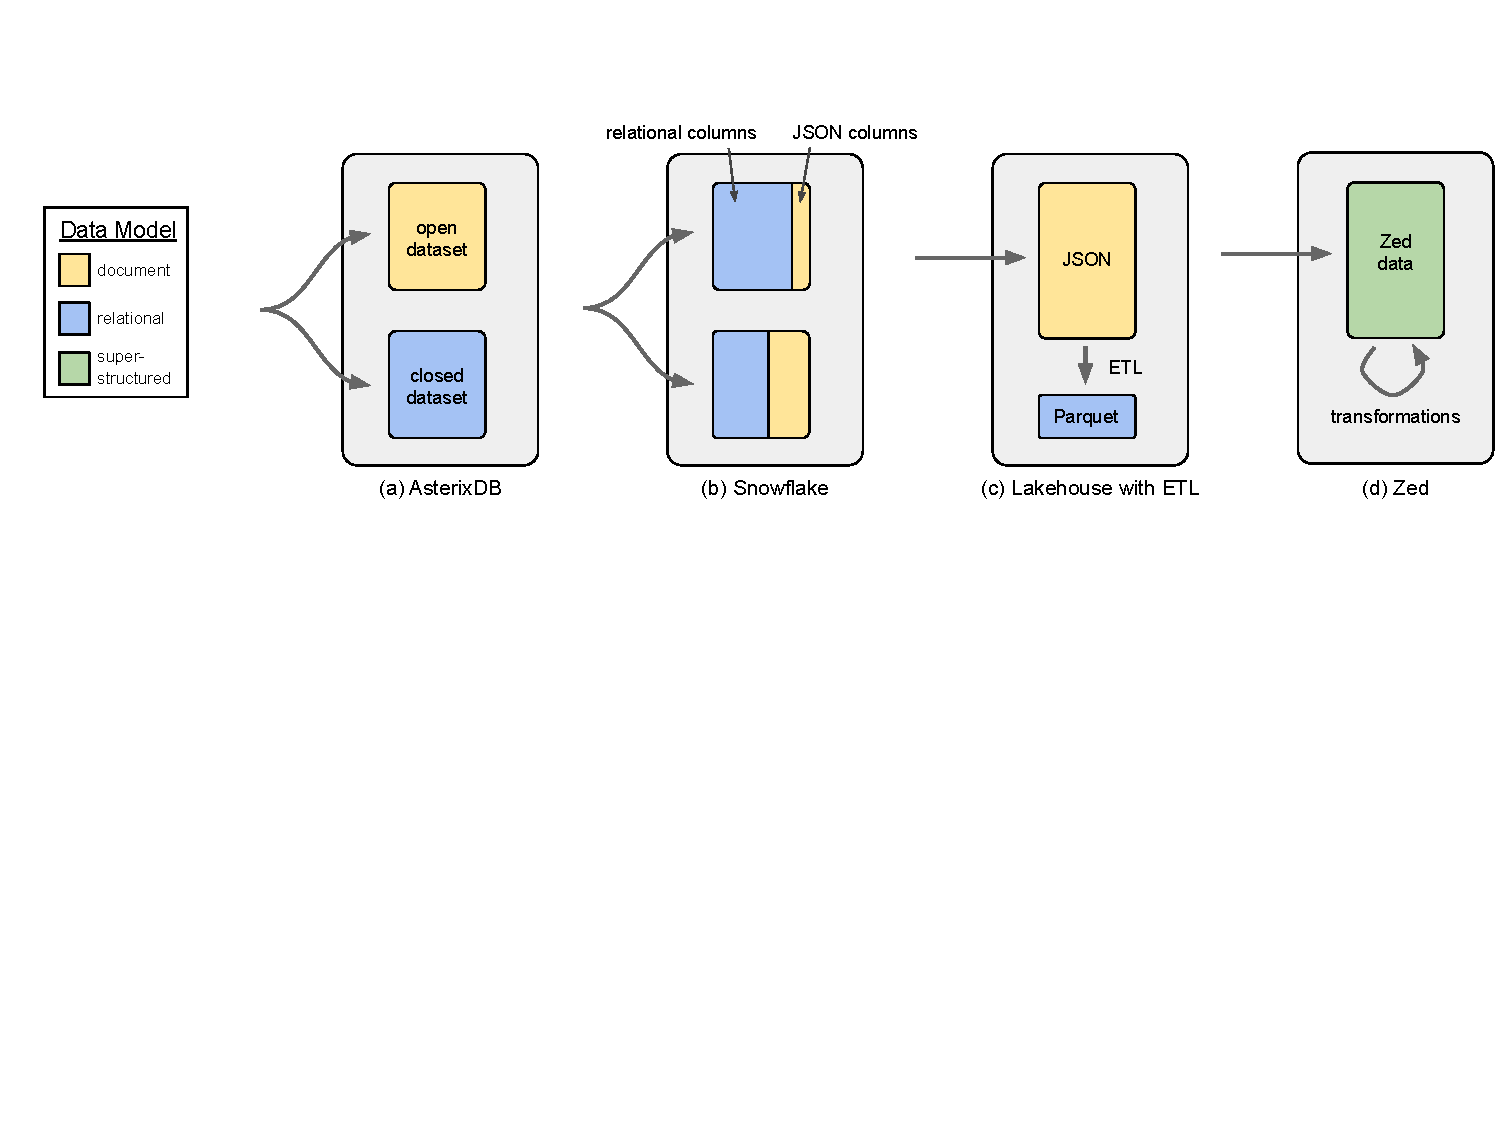
\includegraphics[width=0.81\textwidth]{figures/hybrid_approaches.pdf}
    \vspace{-1.3em}
    \caption{Three example hybrid approaches to data processing: (a) AsterixDB splits incoming data into open and closed datasets in separate files, (b) Snowflake adds columns of JSON data to each relational table, and (c) Lakehouses use ETL to clean a subset of JSON data into Parquet. (d) In Zed, all data (raw or transformed) is represented in the super-structured data model.}
    \label{f:hybrid_approaches}
    \vspace{-1.6em}
\end{figure*}

We start with the observation that what fundamentally enables both efficient analytics and data introspection is knowing the fully specified {\em type} of each piece of data. For example, this allows us to organize and serialized data by type instead of a uniform schema or a relational table.  In this way, a sequence of data conforms to a dynamically defined sum type of all the types present without having to know that sum type {\em a priori}.  Instead, the sum type can be built on the fly as data is each piece of typed data is processed, e.g., in support of streaming workflows.  In contrast, the relational model explicitly requires the set of allowable types (i.e., schemas) to be defined up front, only accepting data from a pre-defined set of schemas across a pre-defined set of tables.  At the other extreme, the document model has no notion of fully-specified types, e.g., the type of the JSON value {\tt \{a:[1,"s"]\}} is simply an "object", whereas in our terminology, its fully specified type is {\em record with field "a" of type array of type union of integer and string}.

Unfortunately, attempts to relax the rigidity of the relational model by integrating the flexibility of the document model have often introduced new problems. For example, some add new external components (e.g., schema registries~\cite{confluent_schema_registry}) that must be integrated with the data processing pipeline, while others incorporate partially typed data (e.g., Snowflake's \texttt{OBJECT} type~\cite{snowflake}) and thus lose some of the benefits of type information.
This leads us to the goal of defining a data model in which every data value has an explicit type and yet there are no constraints on which types are permitted to coexist (e.g., in the same file, table, or set of query results). In other words, our goal is {\em comprehensive yet flexible typing} where both a relational table and a JSON document are simply special cases of the same underlying type-based data model.
%In addition, this type information must be queryable, by which we mean that users can query {\em by} type (e.g., returning all data of a specified type), or \emph{for} type (e.g., returning what types exist in the data set). As we'll see, making types queryable is key to enabling rich data introspection. \noteamy{can we cut the previous 2 sentences? covered by the query language paragraph below}
In addition, this data and its type information should be self-contained so that parsing data never requires coordination with an external registry; instead users can query both data and types in a single unified manner.

%\sr{Needs some connecting tissue here to lead the reader to types as the answer? Can we say something like: We start with the observation that what fundamentally enables both efficient analytics and data introspection is knowing the \emph{type} of data we have. Having type information allows us to, for example, use formats that organize data by type (e.g., by column) for efficent processing, and allows us to reason about the shape of data available (e.g., how many types exist, how many records of each type). The relational model has the well-defined type information that we seek but the problem is it’s overly rigid in its use of this type information — only accepting data from a pre-defined set of types. And attempts to relax this rigidity have introduced new problems — e.g., they add new external components (e.g., schema registries) that require complex integrations with the storage and query processing components, or they resort to weakly defined types (e.g., object) that can’t fully utilize the benefits of types. This leads us to the goal of defining a data model in which all data is typed but that doesn’t constrain what types are permitted. Moreover, this data together with its type information should be self-contained - i.e., the data model must capture both data and their type information in one coherent architecture. These observations lead us to a new data model in which \ldots.} 
%Our unified approach begins with two goals, centered around {\em data types}. First, every data value should have an explicit, queryable type. This enables efficient storage and querying, avoids error-prone schema inference, and enables queries about data types, such as introspection and shaping. At the same time, we should be flexible about which data types are allowed to coexist in the same file, table, or set of query results.
%\noteamy{need to rework the previous 2 paragraphs. they focus too much on limitation 1 and don't really cover 2 or 3.}

%\notesf{I don't find the key idea come through crisply from the current text in the two paragraphs below and I think we should mention schema registries. Let's discuss?}

The key to achieving comprehensive yet flexible typing is to change the way that we associate type information with data values. Instead of associating a single schema with each file or table, which makes it difficult to store or process heterogeneous data together, we propose a new {\em data type abstraction} that is associated directly with individual data values. This enables each value to have an explicit data type (as in the relational model) but also allows different values that are processed together to have different types (as in the document model). We call the resulting data model the {\bf super-structured data model}, because it subsumes the structures of the relational and document data models. Data is organized as a sequence of typed values; when all values have the same type (in the form of a record), this model is equivalent to the relational model.

%\sr{Elaborate? I.e., data is ingested as an ordered stream of typed values. And when all data are the same type, the super-structured model is equivalent to the relational model}\notesf{I strongly agree; I find this a key observation.} 

% \notesf{summarize this by saying ``deep typing without schema rigidity''?} \noteamy{I'm not sure that ``deep typing without schema rigidity'' quite captures the key properties of \sys{}. If we want a summary at that level of detail, what about: ``type flexibility and first-class types''?}

Realizing this approach requires care in designing the type abstraction. We propose an abstraction with the following properties:
\begin{CompactItemize}
    \item Types are {\em associated with individual values}, rather than with a collection such as a table or file.
    \item Types are {\em complete} - we observe that catch-all types such as \texttt{OBJECT} or \texttt{JSON}, or allowing a value to include extra fields beyond those specified by its type prevent the full benefits of types.
    \item Types are {\em first class} - users can query for data types and the query results---which contains types---are returned in the same data model. Users can refer to types by name and data formats can assign numeric type IDs for efficient storage and querying.
    %\item Data types should be {\em identifiable} (i.e., types can be referred to by a numeric ID or string name) - this enables efficient storage and querying because data values can be tagged with their numeric type. It also enables querying values by their type, e.g., to extract all values with a given type, effectively extracting a single relational table from heterogeneous data.
    \item Type definitions are {\em inlined} - this enables data sources to define new types on the fly without out-of-band coordination or additional burden relative to writing JSON data.
\end{CompactItemize}

However, a new data model alone cannot provide the introspection and unification that we seek; we also require a corresponding query language that can exploit the full power of this data model. While the data model encodes per-value type information, the role of the query language is to expose this type information to users. Users should be able to query {\em by} type (e.g., returning all data of a specified type), or \emph{for} type (e.g., returning the type of a data value).
%query {\em for} the type of each individual data value, and to query data values {\em by} type.
In short, types must be {\em first-class members} of the query language as well. This enables rich introspection and is crucial for truly subsuming both the document and relational models. Querying by type allows a user to extract all values with a given schema; the returned data corresponds to a table in the relational model and can be processed as such.



\begin{comment}
\sr{todo. Text that says} 
Data model is only half the story. The other is that we need a corresponding query language that exploits the power of the data model. In our case, this means supporting types as a first-class primitive in the query language - query by type, query for type, operators (compare etc) over types. 
Thus our query language is designed to leverage and complement the properties of the data model: that type information is associated with data, and that this type information is inline with the data (self-contained). 
This enables data introspection. But also allows us to realize the promise that a super-structured data model subsumes both relational and document models. E.g., query by type allows us to extract all records that conform to a particular schema; the returned records correspond to a table in the relational model and can be processed as such.
\end{comment}

In this paper we propose {\bf \sys{}}, a new approach to data processing that is centered around these data types. \sys{} includes a new super-structured data model (\S\ref{ss:zed_data_model}) and query language (\S\ref{ss:zed_query_language}). In addition, \sys{}'s type abstraction allows data to be represented in the format most suitable for the task at hand: columnar for analytics, human-readable for debugging, etc.  Because all data is typed, converting it between formats within the family is lossless and fully automated. Thus \sys{} includes a ``family of data formats'' (\S\ref{ss:zed_formats}). Finally, we will show how \sys{} overcomes the challenges of existing hybrid approaches and unifies the document and relational models in a new way, {\em embodying both at the same time}  (\S\ref{s:zed_in_action}). %\sys{} enables: easy data generation and ingestion, with the ability to create new types on the fly; efficient storage and analytics; data introspection at any stage of data processing; and simplicity, with no dependency on external components such as schema registries (\S\ref{s:zed_in_action}).
